\documentclass[12pt,letterpaper]{article}
\usepackage[utf8]{inputenx} %Codificacion del texto (ISO Latin1 encoding)

\usepackage{fancyhdr} %Permite acomodar a tu gusto la parte de arriba y
% abajo del documento
\usepackage[spanish]{babel} %Permite definir el idioma del dcumento
\usepackage{graphicx} %Permite exportar imagenes en formato eps
\usepackage{url} %Tipo de fuente para correos y paginas
\usepackage{pgf}
\usepackage{fleqn}
\usepackage{amssymb}
\usepackage{amsmath}
\usepackage{fancyvrb}
\usepackage{makeidx}
\usepackage{colortbl} %Permite colocar colores a las tablas
\usepackage{booktabs}
\usepackage[final]{pdfpages}
%%%%%%%%%%
%Margenes%
%%%%%%%%%%
\parskip 1mm %Espacio entre parrafos

\setlength{\topmargin}{0pt}
\topmargin      0.5cm
\oddsidemargin	0.1cm  % Ancho Letter 21,59cm
\evensidemargin 0.5cm  % Alto  Letter 27,81cm
\textwidth	17cm%15.5cm
\textheight	21.0cm
\headsep	4 mm
\parindent	0.5cm
%%%%%%%%%%%%%%%%%%%%%%
%Estilo del documento%
%%%%%%%%%%%%%%%%%%%%%%
\pagestyle{fancyplain}

%%%%%%%%%%%%%%%%%%%%%%%%%%%%%%%%%%%%%%%%%%%
%Fancyheadings. Top y Bottom del documento%
%%%%%%%%%%%%%%%%%%%%%%%%%%%%%%%%%%%%%%%%%%%
% Recuerde que en este documento la portada del documento no posee
% numeracion, pero de igual manera llamaremos a esa primera pagina la numero
% 1, y la que viene la dos. Esto es para tener una idea de las que
% llamaremos pares e impares
\lhead{Investigación de Operaciones I} %Parte superior izquierda
\rhead{\bf \it Tarea 2} %Parte superior derecha
\lfoot{\it } %Parte inferior izquierda. \thepage indica
% el numero de pagina
\cfoot{} %Parte inferior central
\rfoot{\bf \thepage} %Parte inferior derecha
\renewcommand{\footrulewidth}{0.4pt} %Linea de separacion inferior

\newcommand{\primaria}[1]{
	\textbf{\underline{#1}}
}

\newcommand{\foranea}[1]{
	\textbf{\textsl{#1}}
}

\newcommand{\primyfor}[1]{
	\underline{\foranea{#1}}
}

\makeatletter
\newcommand\subsubsubsection{\@startsection {paragraph}{1}{\z@}%
                                   {-3.5ex \@plus -1ex \@minus -.2ex}%
                                   {1.5ex \@plus.2ex}%
                                   {\normalfont\bfseries}}
                       
                                
                                 
\newcommand\subsubsubsubsection{\@startsection {subparagraph}{1}{\z@}%
                                   {-3.5ex \@plus -1ex \@minus -.2ex}%
                                   {1.5ex \@plus.2ex}%
                                  
                                   {\normalfont\bfseries}}


\makeatother
 

\begin{document}
\title{Investigación de Operaciones I \\ \begin{Large}Tarea 2\end{Large}} 
\author{Victor Gonzalez (2.773.029-9)
\and Cesar Muñoz (2.973.053-0)}
\date{\today}
\maketitle


\section{Constructin S.A.}
\subsection{Gráfico de la malla.}
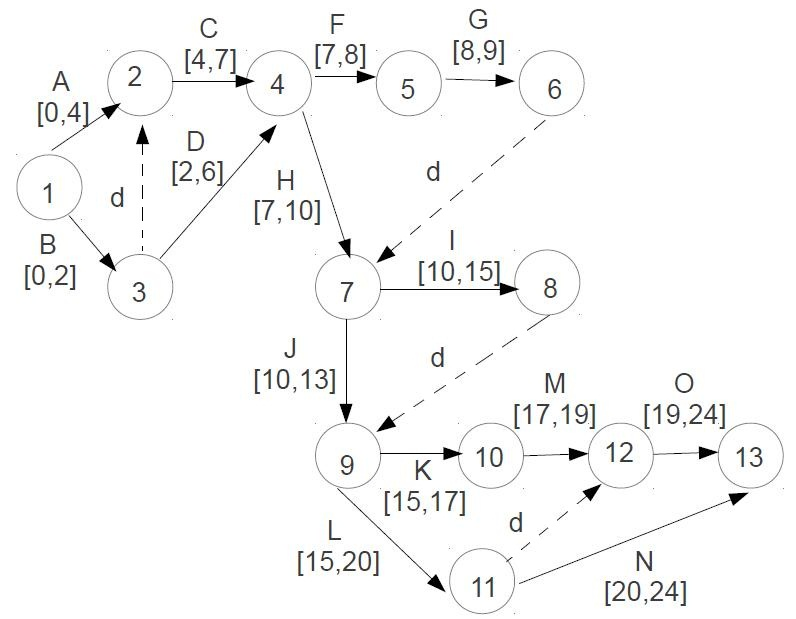
\includegraphics[angle=90]{./src/malla_parte1.jpg}
\subsection{Acelerar el proyecto en 2 días.}
\input{./src/tarea2_parte1.ltx}
\subsection{Programación Lineal en Lp\_Solve.}
\input{./src/tarea2_parte1_costo.ltx}


\section{Novister, conexiones por fibra optica.}
\subsection{Modelo de programación lineal entera.}
\subsubsection{Variables:	}
\begin{description}
\item[Regiones:] I, II, ..., XV, RM. Variables binarias que indican si se instalará una central en la region correspondiente (variables binarias).
\item[Costos Variables:] $C_i$, donde $i={1,\dots,15,RM}$. Representan si se instalaran enlaces adicionales para la región $i$, para cubrir la demanda (variables binarias).
\item[Variable if-else:] Y. Variable que se utiliza para condicionar una situación if-else (variable binaria).
\end{description}

\subsubsection{Función Objetivo:}
$min z = 4 XV + 3 I + 2 II + 5 III + 7 IV + 6 V + 8 RM + 7 VI + 8 VII + 7 VIII + 9 IX + 9 X + 10 XI + 11 XII + 4 XIII + 7 XIV + 2 C_15 + 2 C_1 + 2 C_2 + 2 C_3 + 2 C_4 + 2 C_5 + 2 C_{RM} + 2 C_6 + 2 C_7 + 2 C_8 + 2 C_9 + 2 C_{10} + 2 C_{11} + 2 C_{12} + 2 C_{13} + 2 C_{14}$

\subsubsection{Sujeto a:}
Restricciones de Demanda:
$\\
1800 XV + 1800 I + 400 C15 + 400 C1 + 400 C2 \geq 650 \\
1800 XV + 1800 I + II 1800 + 400 C15 + 400 C1 + 400 C2 \geq 650 \\
1800 I + 1800 II  + 1800 III + 400 C1 + 400 C2 + 400 C3 \geq 700 \\
1800 II + 1800 III + 1800 IV + 400 C2 + 400 C3 + 400 C4 \geq 800 \\
1800 III + 1800 IV + 1800 V + 400 C3 + 400 C4 + 400 C5 \geq 400 \\
1800 IV + 1800 V + 1800 RM + 400 C4 + 400 C5 + 400 CRM \geq 950 \\
1800 V + 1800 RM + 1800 VI + 400 C5 + 400 CRM + 400 C6 \geq 1200 \\
1800 RM + 1800 VI + 1800 VII + 400 CRM + 400 C6 + 400 C7 \geq 600 \\
1800 VI + 1800 VII + 1800 VIII + 400 C6 + 400 C7 + 400 C8 \geq 400 \\
1800 VII + 1800 VIII + 1800 IX + 400 C7 + 400 C8 + 400 C9 \geq 700 \\
1800 VIII + 1800 IX + 1800 X + 400 C8 + 400 C9 + 400 C10 \geq 450 \\
1800 IX + 1800 X + 1800 XI + 400 C9 + 400 C10 + 400 C11 \geq 400 \\
1800 X + 1800 XI + 1800 XII + 400 C10 + 400 C11 + 400 C12 \geq 350 \\
1800 XI + 1800 XII + 1800 XIII + 400 C11 + 400 C12 + 400 C13 \geq 350 \\
1800 XII + 1800 XIII + 1800 XIV + 400 C12 + 400 C13 + 400 C14 \geq 300 \\
1800 XIII + 1800 XIV + 400 C13 + 400 C14 \geq 250 \\
$

Restricciones de distancia (al menos 1 central cada 2 regiones):
$\\XV + I \geq 1 \\
II + III \geq 1 \\
IV + V \geq 1 \\
RM + VI \geq 1 \\
VII + VIII \geq 1 \\
IX + X \geq 1 \\
XI + XII \geq 1 \\
XIII + XIV \geq 1$

$\\
C1 \leq I \\
C2 \leq II \\
C3 \leq III \\
C4 \leq IV \\
C5 \leq V \\
C6 \leq VI \\
C7 \leq VII \\
C8 \leq VIII \\
C9 \leq IX \\
C10 \leq X \\
C11 \leq XI \\
C12 \leq XII \\
C13 \leq XIII \\
C14 \leq XIV \\
C15 \leq XV \\
CRM \leq RM
$

Restricción "Si se construye central en Santiago, no se construye ninguna en V ni en VI":
$\\
V + VI \leq Y \\
RM \leq 1 - Y
$

\subsubsection{Naturaleza de las variables:}
$I, II, III, IV, V, VI, VII, VIII, IX, X, XI, XII, XIII, XIV, XV, RM, Y,\\ C1, C2, C3, C4, C5, C6, C7, C8, C9, C10, C11, C12, C13, C14, C15, CRM, Y \in \{0,1\}$
\subsection{Código LINDO.}
\begin{verbatim}[4]
/* Funcion objetivo */
min: 4 XV + 3 I + 2 II + 5 III + 7 IV + 6 V + 8 RM + 7 VI + 8 VII + 7 VIII + 9 IX + 9 X + 10 XI + 11 XII + 4 XIII + 7 XIV + 2 C15 + 2 C1 + 2 C2 + 2 C3 + 2 C4 + 2 C5 + 2 CRM + 2 C6 + 2 C7 + 2 C8 + 2 C9 + 2 C10 + 2 C11 + 2 C12 + 2 C13 + 2 C14;

/* Restricciones de demanda */
1800 XV + 1800 I + 400 C15 + 400 C1 + 400 C2 >= 650 ;				/* XV Region*/
1800 XV + 1800 I + II 1800 + 400 C15 + 400 C1 + 400 C2 >= 650;		/* I Region */
1800 I + 1800 II  + 1800 III + 400 C1 + 400 C2 + 400 C3 >= 700;		/* II Region */
1800 II + 1800 III + 1800 IV + 400 C2 + 400 C3 + 400 C4 >= 800;		/* III Region */
1800 III + 1800 IV + 1800 V + 400 C3 + 400 C4 + 400 C5 >= 400;		/* IV Region */
1800 IV + 1800 V + 1800 RM + 400 C4 + 400 C5 + 400 CRM >= 950;		/* V Region */
1800 V + 1800 RM + 1800 VI + 400 C5 + 400 CRM + 400 C6 >= 1200;		/* Region Metropolitana*/
1800 RM + 1800 VI + 1800 VII + 400 CRM + 400 C6 + 400 C7 >= 600;	/* VI Region */
1800 VI + 1800 VII + 1800 VIII + 400 C6 + 400 C7 + 400 C8 >= 400;	/* VII Region */
1800 VII + 1800 VIII + 1800 IX + 400 C7 + 400 C8 + 400 C9 >= 700;	/* VIII Region */
1800 VIII + 1800 IX + 1800 X + 400 C8 + 400 C9 + 400 C10 >= 450;	/* IX Region */
1800 IX + 1800 X + 1800 XI + 400 C9 + 400 C10 + 400 C11 >= 400;		/* X Region */
1800 X + 1800 XI + 1800 XII + 400 C10 + 400 C11 + 400 C12 >= 350;	/* XI Region */
1800 XI + 1800 XII + 1800 XIII + 400 C11 + 400 C12 + 400 C13 >= 350;/* XII Region */
1800 XII + 1800 XIII + 1800 XIV + 400 C12 + 400 C13 + 400 C14 >= 300;/* XIII Region */
1800 XIII + 1800 XIV + 400 C13 + 400 C14 >= 250;					/* XIV Region */

/* Restricciones de distancia (al menos 1 central cada 2 regiones) */
XV + I >= 1;
II + III >= 1;
IV + V >= 1;
RM + VI >= 1;
VII + VIII >= 1;
IX + X >= 1;
XI + XII >= 1;
XIII + XIV >= 1;

/* Restricciones de costo: no se pueden usar enlaces
adicionales si no se ha instalado central */
C1 <= I;
C2 <= II;
C3 <= III;
C4 <= IV;
C5 <= V;
C6 <= VI;
C7 <= VII;
C8 <= VIII;
C9 <= IX;
C10 <= X;
C11 <= XI;
C12 <= XII;
C13 <= XIII;
C14 <= XIV;
C15 <= XV;
CRM <= RM;


/* Restriccion if-else: si se hace una central
en RM no se puede construir en V o VI */
/* Si RM > 0 entonces V = VI = 0 */
V + VI <= Y;
RM <= 1 - Y;

/* Naturaleza de las variables */
bin I, II, III, IV, V, VI, VII, VIII, IX, X, XI, XII, XIII, XIV, XV, RM, Y, C1, C2, C3, C4, C5, C6, C7, C8, C9, C10, C11, C12, C13, C14, C15, CRM, Y;
\end{verbatim}

\textbf{Lo cual arroja el siguiente resultado:}
\begin{verbatim}
Value of objective function: 49

Actual values of the variables:
XV                              0
I                               1
II                              1
III                             0
IV                              1
V                               0
RM                              0
VI                              1
VII                             0
VIII                            1
IX                              1
X                               0
XI                              1
XII                             0
XIII                            1
XIV                             0
C15                             0
C1                              0
C2                              0
C3                              0
C4                              0
C5                              0
CRM                             0
C6                              0
C7                              0
C8                              0
C9                              0
C10                             0
C11                             0
C12                             0
C13                             0
C14                             0
Y                               1
\end{verbatim}

\subsection{Definiciones}
\begin{description}
\item[Variable de holgura:] Se utiliza para convertir una desigualdad del tipo $\leq$ en una igualdad simple. Esto se obtiene añadiendo una variable no negativa (por lo general representada por una $S_i$), al lado izquierdo de una restricción, mostrando asi, "que es lo que falta para cumplir la igualdad" de la inecuación.\\
Se refieren tambien a esta variable como la de máximo consumo de un recurso en una solución óptima del problema planteado.
\item[Variable de exceso:] Se utiliza de manera similar a la variable de holgura, pero en este caso para desigualdades del tipo $\geq$. Se representan por una letra $E_i$ por lo general. Estas variables se restan al lado izquierdo de la desigualdad con un valor no negativo.\\
Estas variables representan la cantidad mínima de un recurso que se debe utilizar en la solución óptima.
\item[Variable artificial:] Se usan estas variables cuando se presentan restricciones del tipo $=$ y $\geq$ no contienen al origen dentro de la región factible, por lo que se trata de llevar esas restricciones a una dimensión donde sí se encuentre el origen.\\
Por lo general estas variables se denotan por $A_i$, y no representan nada en especial salvo, llevar la restricción a una región factible del problema.
\end{description}

\bibliographystyle{alpha}
\bibliography{bibbase}

% referencias

\end{document}
